\documentclass[11pt]{article}


%\input{meta/packages}
%
\usepackage{cite}
\usepackage[T1]{fontenc}
\usepackage{times}
\usepackage{url}
\usepackage{amsmath}
\usepackage{fancyhdr}
\usepackage{fancyvrb}
\usepackage{fancybox}
\usepackage{color}
\usepackage{colortbl}
\usepackage[table]{xcolor}
%\usepackage{tex-helpers/mathpartir}
\usepackage{amssymb}
\usepackage{xspace}
\usepackage{comment}
\usepackage{graphicx}
\graphicspath{{figures/}}
\usepackage{epsfig}
\usepackage{wrapfig}
\usepackage{multirow}
\usepackage{subfig}

% Added listing for code listings
\usepackage{listings}
\usepackage{relsize}
\usepackage{setspace}
\usepackage{sidecap}
\usepackage{algorithm}
\usepackage{algorithmic}

\textwidth=16.5cm 
\textheight=22.5cm 
\textwidth=16.5cm 
\textheight=55.5pc
\topmargin=-0.5cm 
\headsep=0cm 
\headheight=0cm 
\oddsidemargin=0cm
\evensidemargin=0cm 
\marginparwidth=0cm
\parskip=0cm
\itemsep=0.1pt
\parindent=0.5cm

%Set table separation 
\setlength{\tabcolsep}{1pt}

% Allow figures to take up the entire page
\renewcommand\floatpagefraction{.99}
\renewcommand\topfraction{.99}
\renewcommand\bottomfraction{.90}
\renewcommand\textfraction{.01}   
\setcounter{totalnumber}{50}
\setcounter{topnumber}{50}
\setcounter{bottomnumber}{50}

% formatting for grammars
%\input{tex-helpers/obey}
%\input{tex-helpers/grammar}
%\renewcommand{\nonterm}[1]{\mbox{\textit{#1}}}
\newcommand{\oneormore}[1]{#1\ensuremath{^+}}

\newcommand{\opt}[1]{\textbf{[}#1\textbf{]}}

\newcommand{\mc}[1]{\mbox{\rm \ensuremath{\text{\code{#1}}}}} 
\newcommand{\loc}{\ensuremath{\mathord{\mathit{loc}}}}
\newcommand{\ec}{\ensuremath{\mathop{\mathbb{E}}}}
\newcommand{\hole}{\ensuremath{\mathord{\mathit{-}}}}
\newcommand{\reducesto}{\hookrightarrow}

\newcommand*{\seq}[1]{\ensuremath{\left\langle {#1} \right\rangle}}
\newcommand{\config}{\seq}
\newcommand{\udot}{\mathbin{\sqcup \kern-0.53em \cdot \,}}

% Aux functions
\newcommand{\auxFunc}[1]{\ensuremath{\mathop{\mathit{#1}}}}
\newcommand{\concat}{\auxFunc{concat}}
\newcommand{\reverse}{\auxFunc{reverse}}

% Type checking macros
% change symbol type of : from mathrel 
%\DeclareMathSymbol{:}{\mathbin}{operators}{"3A} 
\newcommand{\OK}{\mbox{OK}}
\newcommand{\OKin}{\mbox{OK in }}
\newcommand{\isType}{\mbox{\textit{isType}}}
\newcommand{\isThunkType}{\mbox{\textit{isThunkType}}}
\newcommand{\isClass}{\mbox{\textit{isClass}}}
\newcommand{\Types}{\mbox{\textit{Types}}}
\newcommand{\Names}{\mbox{\textit{Names}}}
\newcommand{\TypeEnv}{\mbox{\textit{TypeEnv}}}
\newcommand{\VD}{\mbox{\textit{VD}}}
\newcommand{\TypesInOrder}{\mbox{\textit{typesInOrder}}}
\newcommand{\dom}{\mbox{\textit{dom}}}
\newcommand{\rng}{\mbox{\textit{rng}}}
\newcommand{\POWERSET}[1]{\mbox{\textit{PowerSet}}(#1)}
\newcommand{\delete}{\mbox{\textit{delete}}}
\newcommand{\mklist}{\mbox{\textit{mksupers}}}
\newcommand{\uminus}{\mbox{$\cup\!\!\!\!-$}}
\newcommand{\iminus}{\mbox{$\cap\!\!\!\!-$}}
\newcommand{\rname}[1]{$\TirName{(#1)}$} % for inline inferrule names
\newcommand{\STO}{\ensuremath{<:}}  % ``subtype of''
\newcommand{\consistent}{\ensuremath{\approx}}

% Notations 
\newcommand{\produces}{\rightsquigarrow}
\newcommand{\refinedBy}{\sqsubseteq}

% Macros for the Figure Editor Example
\newcommand{\FElement}{\mbox{\texttt{FElement}~}}
\newcommand{\ChangedFE}{\mbox{\texttt{changedFE}~}}
\newcommand{\FEChange}{\mbox{\texttt{FEChange}~}}


% Macros for defining phase transition analysis
\newcommand{\cfg}{\ensuremath{{\cal CFG}}\xspace}
\newcommand{\globTypeMap}{\ensuremath{T}\xspace}

%Redefinition of some math commands widely used outside
%mathmode
\newcommand{\memOf}{\ensuremath{\in}\xspace}

% Help LaTeX not violate the column margins
\tolerance=50000

% settings for listings
\definecolor{lightgray}{gray}{0.97}
\definecolor{darkgray}{gray}{0.5}
\definecolor{OliveGreen}{cmyk}{0.64,0,0.95,0.40}
\definecolor{DarkGreen}{cmyk}{0.58,0,0.66,0.26}
\definecolor{LightRed}{cmyk}{0,0.682,0.728,0}
\definecolor{purple}{cmyk}{0.41,0.73,0,0}

\lstset{
	language=bash, emph={},
	mathescape=false, escapechar=@,
	backgroundcolor=\color{lightgray},
	commentstyle=\color{darkgray},
	keywordstyle=\color{OliveGreen}\bfseries,
	basicstyle=\relsize{-3}\sffamily,
	numberstyle=\scriptsize\sffamily,
	emphstyle=\color{purple},
	emphstyle={[2]\color{LightRed}},
	commentstyle=\color{DarkGreen},
	stringstyle=\color{OliveGreen},
	numbers=left, stepnumber=1,
	numberblanklines=false,
	numberstyle=\tiny,
	numbersep=-3pt,
	frame=none, framexleftmargin=0pt, framexrightmargin=0pt, 
	%xleftmargin=15pt, xrightmargin=4pt,
	columns=flexible, breaklines=true,
	showspaces=false, showstringspaces=false, showtabs=false, tabsize=2,
	morekeywords={input,exists,foreach,ifall,output,of,weight,stop,visit,before,after},
	emph={int,string,bool,time,array,stack,map,visitor,%
true,false,%
top,sum,mean,maximum,minimum,set,collection,%
Project,CodeRepository,Revision,ChangedFile,ASTRoot,Namespace,Declaration,Type,Method,Variable,Statement,Expression,Modifier,%
ExpressionKind,NEW,LITERAL,EQ,NEQ,%
TypeKind,CLASS,ANONYMOUS,%
ModifierKind,OTHER,%
ChangeKind,DELETED,%
StatementKind,IF,%
RepositoryKind,SVN},
	emph={[2]isfixingrevision,getast,iskind,hasfiletype,isliteral,getsnapshot,has_modifier_public,%
format,def,len,match,lowercase,yearof,haskey,remove,strfind,push,pop},
}

% could use \relsize{-2} instead of \scriptsize below
\newcommand{\FIGCODEFONT}{\relsize{-2.5}\ttfamily}

% cross referencing
%\newcommand{\algref}[1]{Algorithm~\ref{#1}}
%\newcommand{\figref}[1]{Figure~\ref{#1}\xspace}
%\newcommand{\tabref}[1]{Table~\ref{#1}\xspace}
%\newcommand{\fignref}[1]{Figure~\ref{#1}\xspace}
%\newcommand{\secref}[1]{Section~\ref{#1}\xspace}
%\newcommand{\secnref}[1]{Section~\ref{#1}\xspace}

%\newcommand{\etal}{~\textit{et al.}\@\xspace}
\newcommand{\kind}{\textit{kind}\xspace}
\newcommand{\KIND}{\textit{KIND}\xspace}

\newcommand{\lang}{\textit{Boa}\@\xspace}

% Theorems environments...
%{theorems}
\newtheorem{theorem}{Theorem}[section]
\newtheorem{axiom}[theorem]{Axiom}
\newtheorem{corollary}[theorem]{Corollary}
\newtheorem{definition}[theorem]{Definition}
\newtheorem{example}[theorem]{Example}
\newtheorem{fact}[theorem]{Fact}
\newtheorem{lemma}[theorem]{Lemma}
\newtheorem{proposition}[theorem]{Proposition}
\newtheorem{remark}[theorem]{Remark}
\newtheorem{conjecture}[theorem]{Conjecture}
% Some helpful notation
\newcommand{\PROOF}{{\em Proof:\/}~~}
\newcommand{\PROOFSKETCH}{{\em Proof Sketch:\/}~~}
\newcommand{\QED}{\rule{0.4em}{0.65em}}

\definecolor{light-gray}{gray}{0.9}
\definecolor{very-light-gray}{gray}{0.95}

% Change section headings to look nicer
\makeatletter
\renewcommand\thesection{{\large\Alph{section}.}}
\renewcommand\section{\@startsection {section}{1}{\z@}%
                                   {-3.5ex \@plus -1ex \@minus -.2ex}%
                                   {2.3ex \@plus.2ex}%
                                   {\large\scshape\bf}}
\makeatother

\renewcommand\thesubsection{{\normalsize\Alph{section}.}{\normalsize\arabic{subsection}}}

\makeatletter
\renewcommand\subsection{\@startsection {subsection}{1}{\z@}%
                                   {-3.5ex \@plus -1ex \@minus -.2ex}%
                                   {2.3ex \@plus.2ex}%
                                   {\normalsize\scshape\bf}}
\makeatother

\renewcommand\thesubsubsection{{\normalsize\Alph{section}.}{\normalsize\arabic{subsection}.}{\normalsize\arabic{subsubsection}}}

\makeatletter
\renewcommand\subsubsection{\@startsection {subsubsection}{1}{\z@}%
                                   {-3.5ex \@plus -1ex \@minus -.2ex}%
                                   {2.3ex \@plus.2ex}%
                                   {\normalsize\scshape\bf}}
\makeatother

\newcommand\para[1]{\vspace{-1em}\paragraph{#1\ }}

% Different font in captions
\newcommand{\captionfonts}{\footnotesize}

% formatting of initial section quotations
\newcommand{\QUOTATION}[1]{\begin{flushright}\begin{footnotesize}\emph{#1}\end{footnotesize}\end{flushright}}
 
\makeatletter  % Allow the use of @ in command names
\long\def\@makecaption#1#2{%
  \vskip\abovecaptionskip
  \sbox\@tempboxa{{\captionfonts #1: #2}}%
  \ifdim \wd\@tempboxa >\hsize
    {\captionfonts #1: #2\par}
  \else
    \hbox to\hsize{\hfil\box\@tempboxa\hfil}%
  \fi
  \vskip\belowcaptionskip}
\makeatother   % Cancel the effect of \makeatletter

%\usepackage[ps2pdf,bookmarks=true]{hyperref}

\definecolor{light-gray}{gray}{0.9}
\definecolor{dark-gray}{gray}{0.7}

\newcommand\doctitle[1]{\newpage \setcounter{page}{1}\thispagestyle{fancyplain} \headheight=14pt%
                        \fancyhead[C]{\large{\bf #1}}\xspace\vspace{0.5em}}


                                                                        


\usepackage{graphicx,times}
\usepackage{wrapfig}
\usepackage{amsmath,epsfig}
\usepackage{setspace,array}
\usepackage{cite}
\usepackage{listings}
\usepackage{booktabs}
%\usepackage{bibentry}
\lstset{basicstyle=\scriptsize\sffamily,language={},frame=single,breaklines=true,columns=fullflexible,mathescape=true,escapechar=@}

\usepackage{tikz}
\newcommand*\circled[1]{\tikz[baseline=(char.base)]{
		\node[shape=circle,draw,inner sep=0.45pt] (char) {#1};}}


\usepackage{xspace}

\usepackage{sectsty}
\sectionfont{\large}
\subsectionfont{\normalsize}
\subsubsectionfont{\normalsize}

\usepackage[compact]{titlesec}

\renewcommand{\theequation}{\thesection.\arabic{equation}}
\renewcommand{\baselinestretch}{1.0}

\newcommand*\rotdia{\multicolumn{1}{R{45}{1em}}}% no optional argument here, please!
\newcommand*\rot{\rotatebox{90}}
\usepackage{multicol,multirow}

\newtheorem{Definition}{Definition}
\newtheorem{Claim}{Claim}
\newtheorem{Lemma}{Lemma}
\newtheorem{Theorem}{Theorem}
\newtheorem{Property}{Property}
\newtheorem{Problem}{Problem}


\newcommand\aName[1]{{\small\textsc{#1}}\xspace}

% cross referencing
\newcommand{\figref}[1]{Figure~\ref{#1}}
\newcommand{\secref}[1]{Section~\ref{#1}}
\newcommand{\tabref}[1]{Table~\ref{#1}}
\newcommand{\defref}[1]{Definition~\ref{#1}}

%\newcommand\aName[1]{{\small\textnormal{\textsc{#1}}}\xspace}

%\newcommand\MUBench[0]{\aName{MuBench}}
\newcommand\MUDetect[0]{\aName{MuDetect}}



\newcommand\MUBench[0]{\aName{MuBench}}
\newcommand\MUPipe[0]{\aName{MuPipe}}
\newcommand\MUC[0]{\aName{MuC}}
\newcommand\AUG[0]{\aName{AUG}}

\newcommand{\etal}{{\em et al.}}

\newcommand\GROUM[0]{\aName{GROUM}}
\newcommand\eGROUM[0]{\aName{AUG}}
\newcommand\miner[0]{\aName{AUGMiner}}

\newcommand\Colibri[0]{\aName{Colibri/ML}}
\newcommand\DroidAssist[0]{\aName{DroidAssist}}
\newcommand\GraPacc[0]{\aName{GraPacc}}
\newcommand\GROUMiner[0]{\aName{GROUMiner}}
\newcommand\Jadet[0]{\aName{Jadet}}
\newcommand\PRMiner[0]{\aName{PR-Miner}}
\newcommand\CARMiner[0]{\aName{CAR-Miner}}
\newcommand\Alattin[0]{\aName{Alattin}}
\newcommand\Tikanga[0]{\aName{Tikanga}}
\newcommand\DMMC[0]{\aName{DMMC}}
\newcommand\RGJ[0]{\aName{RGJ07}}
\newcommand\Chronicler[0]{\aName{Chronicler}}
\newcommand\Acharya[0]{\aName{AX09}}

\newcommand{\checkNum}[1]{#1}

\newcommand{\revise} {\bf}

\newcommand{\code}[1]{{\scriptsize\texttt{#1}}}
\newcommand{\op}{\tau}
\newcommand{\refac}{\rho}
\newcommand{\edit}{\sigma}
\newcommand{\T}{\theta}
\newcommand{\comp}{;}
\newcommand{\pre}{\prec_P}
\newcommand{\meth}{KSISA}

\newcommand{\MyParagraph}[1]{\textbf{#1}{ }}
\newcommand{\fixme} [1] {\textcolor{red}{{\it FIXME}: #1}}

\usepackage{vmargin}
\setpapersize{USletter}
\setmarginsrb{1.0in}{1in}{1.0in}{1in}%
           {0pt}{0mm}{0pt}{10mm}
\newcommand{\remove}[1]{}



\usepackage{tweaklist}
\renewcommand{\enumhook}{\setlength{\topsep}{0pt}%
  \setlength{\itemsep}{0pt}}
\renewcommand{\itemhook}{\setlength{\topsep}{0pt}%
  \setlength{\itemsep}{0pt}}
\renewcommand{\descripthook}{\setlength{\topsep}{0pt}%
  \setlength{\itemsep}{0pt}}



%\newcommand\Tone{Thrust 1 (T1). Ongoing Evaluation of Existing Code Representation Learning in Bug Detect-Fix Processes}
\newcommand\Tone{Thrust 1 (T1). Design Framework and Environment for Code Representation Learning (CRL): Representations, Models, and Methodologies}

\newcommand\Ttwo{Thrust 2 (T2). Quality Evaluation Framework for Code Representation Learning}

\newcommand\Tthree{Thrust 3 (T3). Applications of CRL Framework in Bug Detection, Testing, Fault Localization, and Auto Program Repair}

%Enhancing Techniques in the Bug Fixing Process with Deep Learning}

% all tool names used in this proposal

%\newcommand\tool{NeuralPPA}

\newcommand{\tool}{\textsc{NeuralPDA}\xspace}

\newcommand\deepbugs{\textbf{DeepBugs}~\cite{Pradel-2018}}
\newcommand\bugram{\textbf{Bugram}~\cite{Wang-2016}}
\newcommand\narminer{\textbf{NAR-miner}~\cite{Bian-2018}}
\newcommand\findbugs{\textbf{FindBugs}~\cite{ayewah-2007}}
\newcommand\deepsim{\textbf{DeepSim}\cite{Zhao-2018}}
\newcommand\codetovec{\textbf{code2vec}\cite{Alon-2018}}
\newcommand\codevectors{\textbf{CodeVectors}\cite{Henkel-2018}}
\newcommand\dlsim{\textbf{DL-Sim}~\cite{Tufano-2018}}
\newcommand\treelstm{\textbf{Tree~LSTM}~\cite{Tai-2015}}

\newcommand\cnn{CNN~\cite{kim2014convolutional}}



% auto-fix
\newcommand\CODIT{\textbf{CODIT}~\cite{chakrabortycodit}}
\newcommand\Ratchet{\textbf{Ratchet}~\cite{hata2018learning}}
\newcommand\Tufano{\textbf{Tufano}~\cite{tufano2019learning}}
\newcommand\CoCo{\textbf{CoCoNut}~\cite{lutellier2020coconut}}

% FL
\newcommand\MLP{\textbf{MLP}~\cite{bourlard1988auto}}

%%%%%%%%%%%%%%%%%%%%%%%%%%%%%%%
%\usepackage{pgfgantt}
%\definecolor{barblue}{RGB}{153,204,254}
%\definecolor{groupblue}{RGB}{51,102,254}
%\definecolor{linkred}{RGB}{165,0,33}
%\renewcommand\sfdefault{phv}
%\renewcommand\mddefault{mc}
%\renewcommand\bfdefault{bc}
%\sffamily
%%%%%%%%%%%%%%%%%%%%%%%%%%%%%%%

\usepackage{array}
\usepackage{ragged2e}
%\newcolumntype{L}[1]{>{\raggedright\arraybackslash\hspace{0pt}}p{#1}}
\newcolumntype{L}[1]{l}
\newcolumntype{C}[1]{>{\centering\arraybackslash}p{#1}}

\usepackage[colorlinks=true, urlcolor=blue]{hyperref}


\begin{document}

\begin{center}
{\large \bf Enabling Partial Program Dependence Analysis Using Neural Networks}
\end{center}
\vspace{-.1in}
\hrule

\vspace{1em}
Principal Investigator: Dr. Tien N. Nguyen

\hspace{9em} \textit{Professor}

\hspace{9em} \textit{Erik Johnson School of Engineering and Computer Science}

\hspace{9em} \textit{The University of Texas at Dallas}
%Co-PI: <PI name>, <title>, <department name>, <university name>

Cash Funding Needed: \$80,000
%AWS Promotional Credits needed: 

Amazon Contact: Dr. Hoan Anh Nguyen, \href{mailto:nguyenanhhoan@gmail.com}{\em nguyenanhhoan@gmail.com}

\vspace{0.5em}

\noindent {\bf \textit{Abstract}.} Code fragments from developer forums often migrate to applications due to the code reuse practice. Owing to the limitation of current program analysis (PA) tools of only being able to analyze complete code, analyzing the incomplete code fragments to early determine the presence of potential vulnerabilities is challenging. Previous studies have demonstrated lexical, syntactic, and semantic repetitiveness of source code in open-source projects. In this proposal, we seek to address these issues as follows: (a) create benchmark CFG/PDG datasets of varying maturity levels; (b) develop a neural network-based program dependence learning infrastructure to predict CFG/PDGs for both complete and partial code fragments; (c) utilize the predicted CFG/PDGs to establish a pipeline to predict vulnerabilities in incomplete code fragments.

\vspace{0.25em}
\noindent {\bf \textit{Keywords}.} partial program dependence analysis, vulnerability detection 
\vspace{0.5em}

\section{Introduction}
%% Introduction
Developers often use online question and answering (Q\&A) forums, e.g., StackOverflow (S/O), to learn how to use software libraries and frameworks. Sometimes, the answer to a question comes as a fragment/chunk of code, which later makes it to the production applications, stemming from the copy-and-paste software reuse practice. Unfortunately, if the copied code fragments are vulnerable, i.e., possess defects that can potentially be exploited, it will lead to the applications being prone to attacks. Verdi et al.~\cite{verdi-tse22} reviewed more than 72K C++ code snippets that migrated from 1,325 S/O answers. Of these, they reported a total of 99 vulnerable code snippets of 31 different types that made their way to 2,589 GitHub repositories. Thus, it is crucial to detect early the vulnerabilities in the code snippets from online forums.

%BufferOverFlow,SQLInj,Cross-siteScripting,AuthBypassSpoofing

Security researchers have proposed several automated approaches for vulnerability detection (VD) in software systems using program analysis (PA)~\cite{FlawFinder,RATS,viega2000its4,Checkmarx,HPFortify,Coverity}, as well as machine and deep learning (ML \& DL)~\cite{fse21,chakraborty2020deep,zhou2019devign,li2018sysevr,li2018vuldeepecker} techniques. These approaches typically leverage program representations such as the control-flow graph (CFG)~\cite{fse21} and program dependence graph (PDG)~\cite{fse21} to succinctly represent all execution flows and the data-flow information in the program, so as to model/describe the vulnerable features. However, the PA tools employed to derive these program representations warrant the code to exist as complete program units, at the very least, at the method-level granularity. This makes it impossible to utilize such VD tools to find vulnerabilities in code snippets. A possible alternative would be to plug the code snippet into the method, resolve any ambiguities, and test it with a VD tool. However, such a strategy is limited. First, if found vulnerable, the efforts of integrating the code snippet into the existing method would be lost. Second, due to the black-box nature of DL models, we would not know the origin of the vulnerability, i.e., whether it arises due to the flawed code snippet or the existing part of the code.

Besides, analyzing code snippets is not straightforward as they are often incomplete, un-parseable, contain declaration/reference ambiguity, and are interspersed between user comments. Currently, there exist tools such as PPA~\cite{ppa08},~which parse an incomplete code fragment to build the AST and~ex\-tract data types in a best-effort manner, while StatType \cite{icse18} resolves the libraries and recovers only the fully-qualified names for references. However, deriving the program dependencies on incomplete code snippets is not yet possible. Let us call such an analysis, {\em partial program dependence analysis}.

In addition to vulnerability detection, such partial program dependence analysis is also beneficial to the other software engineering (SE) tasks that can tolerate a low level of errors and imprecision in building the dependencies. For example, consider code completion~\cite{codefill-icse22,facebook-icse21}, in which a model provides suggestions to complete partial code. Existing ML/DL-based code completion models are just based on the code sequences or utilize the syntactic structure in ASTs, but none leverage the program dependencies due to the nature of partial code. Next, consider the task of analyzing the code fragments in a bug report to connect it to the relevant source files for bug localization purposes~\cite{euler-fse19,icpc17}. Here too, a need for partial program dependence analysis can be observed.


%% Research Objectives
\subsection{Research Objectives}
While the state-of-the-art research and practice has been well-established for deriving control-flow and program dependencies for entire programs, there have been little to no advancements in conducting such a program dependence analysis for partial programs. In this proposal, we set out to investigate and develop {\tool}, a {\em \underline{Neural} Network-Based \underline{P}rogram \underline{D}ependence \underline{A}nalysis} infrastructure, that enables (partial) program dependence analysis. Besides, leveraging one such neural network-based approach will help gain a significant time markup in dependency discovery in contrast to traditional program analysis tools.


\begin{center}
    \begin{minipage}{33.5em}
    The key philosophy that drives our work is that {\em the dependence analysis of partial code can be learned from the dependence analysis for entire programs via the wealth of information obtained from ultra-large-scale, open-source software repositories}.
    \end{minipage}
\end{center}


We draw motivation for such a data-driven, learning-based approach from the following. First, ultra-large-scale software repositories, e.g. GitHub (7M+ projects) and SourceForge (700k+ projects) contain an enormous collection of programs. These repositories amount to 1B+ lines of code, 10M+ revision logs, and 3M+ issue reports. This wealth of knowledge is an excellent source for {\tool}. Hindle {\em et al.}~\cite{} have shown that code has high repetitiveness and predictability, and can be captured well by statistical models. Thus, we expect to build ML/DL models to learn from those repositories. Second, in an empirical study on the repetitiveness, containment, and composability of PDGs in open-source projects, the PI group~\cite{} reported that among 17.5M PDGs with 1.6B PDG subgraphs, 14.3\% of the PDGs have all of their subgraphs repeated across different projects. Furthermore, in 15.6\% of the PDGs, at least 90\% of their subgraphs are likely to have appeared before in other projects. Thus, {\tool} could learn from PDGs with complete program dependencies retrieved from existing code repositories and derive the dependencies for the (partial) code fragment under study. Broadly, such a partial program dependence analysis infrastructure is similar in spirit to neural network-based dependency parsing approaches in natural language processing (NLP), which learn the dependencies signifying the semantic relationships between words in a sentence from the text corpora.

We propose the following thrusts of research:

\vspace{3pt}
\noindent \textbf{[Thrust 1] Lorem}

\vspace{3pt}
\noindent \textbf{[Thrust 2] Neural Network-Based Program Dependence Analysis Infrastructure.} The basic infrastructure has two main tasks. First, it learns the well-defined syntactic and semantic information in source code by leveraging the program representations obtained for the complete programs in the training dataset, collected from large-scale code repositories. Next, one such trained model infers the program dependencies among the statements in any given code fragment, either complete or partial code.

\vspace{3pt}
\noindent \textbf{[Thrust 3] Enabling Fragment-Level Vulnerability Detection with \tool.} Vulnerability detection in code fragments can be facilitated as follows: (a) employing \tool infrastructure to predict the CFG/PDG for a given code fragment; (b) leveraging an existing automated VD tool that utilizes the predicted CFG/PDGs to identify the presence of vulnerabilities in partial code fragments.


%% Methodology
\subsection{Methodology}
\begin{itemize}
    \item {\bf Task A.} Collect high-quality, compilable Java and C/C++ programs and extract PDG/CFGs.
    \item {\bf Task B.} Design preliminary model to predict inter-statement control-flow and program dependencies.
    \item {\bf Task C.} Implement model and design experiments for both qualitative and quantitative evaluation.
    \item {\bf Task D.} Leverage automated vulnerability detection tool to identify vulnerable code fragments.
    \item {\bf Task E.} Model testing, tool release, and manuscript dissemination.
\end{itemize}

\begin{figure}[h]
    \centering
    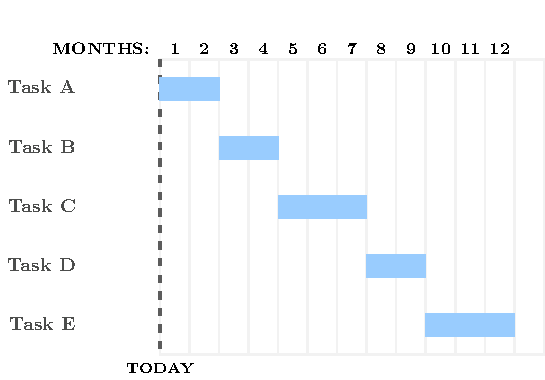
\includegraphics{gannt_charts/gannt.pdf}
    \caption{Anticipated Timeline}
    \label{fig:timeline}
\end{figure}

% Please add the following required packages to your document preamble:
% \usepackage[table,xcdraw]{xcolor}
% If you use beamer only pass "xcolor=table" option, i.e. \documentclass[xcolor=table]{beamer}
\begin{table}[]
\begin{tabular}{|ccc|}
\hline
\multicolumn{3}{|c|}{\cellcolor[HTML]{343434}{\color[HTML]{FFFFFF} \textbf{Project Milestones \& Deliverables}}}                                                                     \\ \hline\hline
\multicolumn{3}{|c|}{\textbf{T1. Benchmark Dataset Construction}}                                                                                                                    \\ \hline
\multicolumn{1}{|p{1cm}|}{\textbf{1.1}} & \multicolumn{1}{c|}{Collect high-quality, compilable Java and C/C++ programs and extract PDG/CFGs.}                           & Months 1 -- 2   \\ \hline\hline
\multicolumn{3}{|c|}{\textbf{T2. NeuralPDA Infrastructure}}                                                                                                                          \\ \hline
\multicolumn{1}{|p{1cm}|}{\textbf{2.1}} & \multicolumn{1}{c|}{Design and implement preliminary model to predict inter-statement control-flow and program dependencies.} & Months 3 -- 4   \\
\multicolumn{1}{|p{1cm}|}{\textbf{2.2}} & \multicolumn{1}{c|}{Enhance preliminary model and design experiments for both qualitative and quantitative evaluation.}       & Months 5 -- 7   \\ \hline\hline
\multicolumn{3}{|c|}{\textbf{T3. Fragment-Level Vulnerability Detection}}                                                                                                            \\ \hline
\multicolumn{1}{|p{1cm}|}{\textbf{3.1}} & \multicolumn{1}{c|}{Leverage automated vulnerability detection tool to identify vulnerable code fragments.}                   & Months 8 -- 9   \\
\multicolumn{1}{|p{1cm}|}{\textbf{3.2}} & \multicolumn{1}{c|}{Model testing, benchmark dataset and tool release, and manuscripts dissemination.}                        & Months 10 -- 12 \\ \hline
\end{tabular}
\end{table}

%% Preliminary Work
\subsection{Preliminary Work}
%Toward this theme, in our preliminary work, we developed DeepPDA, a neural network-based partial program dependence analysis approach that learns to derive the program dependencies for any code fragments (i.e., both complete and incomplete). In our preliminary empirical evaluation, we intrinsically evaluated it on Java and C/C++ programs. First, we trained {\tool} on complete code. For testing, we treated each method individually and chose a consecutive portion within the method to predict the program dependencies, and compared them against the actual dependencies. Overall, DeepPDA predicts CFG and PDG edges in Java with an F-score of 94.29\%, and in C++ with an F-score of 92.46\%.


In Figure~\ref{fig:model}, we present a preliminary design of the general architecture of \tool model. Given that attention is the driver behind the now ubiquitous Transformers’~\cite{Vaswani-2017} success in efficiently learning representations for different entities in different contexts, we plan to make it the foundation of the context learning components in our model as well. Each is intended to learn different aspects of contextualization. For our preliminary empirical evaluation, we collected Java methods from the GitHub Java Corpus~\cite{githubCorpus2013} and generated their CFG/PDGs using Joern program analysis tool~\cite{joern-2014}. By employing a self-attention network for both intra-statement and inter-statement contextualization, we trained a bootstrap model on complete code. For testing, we treated each method individually and chose a consecutive portion within the method to predict the program dependencies, and compared them against the actual dependencies. Overall, our bootstrap model was able to predict CFG and PDG edges in Java programs with an F-score of 94.29\%.


%% Anticipated Results
\subsection{Anticipated Results}
In Table~\ref{tab:milestones}, we detail a one-year schedule breakdown for various tasks associated with all research axes, and the anticipated timeframe to reach the set milestones.
% Please add the following required packages to your document preamble:
% \usepackage[table,xcdraw]{xcolor}
% If you use beamer only pass "xcolor=table" option, i.e. \documentclass[xcolor=table]{beamer}
\begin{table}[]
\begin{tabular}{|ccc|}
\hline
\multicolumn{3}{|c|}{\cellcolor[HTML]{343434}{\color[HTML]{FFFFFF} \textbf{Project Milestones \& Deliverables}}}                                                                     \\ \hline\hline
\multicolumn{3}{|c|}{\textbf{T1. Benchmark Dataset Construction}}                                                                                                                    \\ \hline
\multicolumn{1}{|p{1cm}|}{\textbf{1.1}} & \multicolumn{1}{c|}{Collect high-quality, compilable Java and C/C++ programs and extract PDG/CFGs.}                           & Months 1 -- 2   \\ \hline\hline
\multicolumn{3}{|c|}{\textbf{T2. NeuralPDA Infrastructure}}                                                                                                                          \\ \hline
\multicolumn{1}{|p{1cm}|}{\textbf{2.1}} & \multicolumn{1}{c|}{Design and implement preliminary model to predict inter-statement control-flow and program dependencies.} & Months 3 -- 4   \\
\multicolumn{1}{|p{1cm}|}{\textbf{2.2}} & \multicolumn{1}{c|}{Enhance preliminary model and design experiments for both qualitative and quantitative evaluation.}       & Months 5 -- 7   \\ \hline\hline
\multicolumn{3}{|c|}{\textbf{T3. Fragment-Level Vulnerability Detection}}                                                                                                            \\ \hline
\multicolumn{1}{|p{1cm}|}{\textbf{3.1}} & \multicolumn{1}{c|}{Leverage automated vulnerability detection tool to identify vulnerable code fragments.}                   & Months 8 -- 9   \\
\multicolumn{1}{|p{1cm}|}{\textbf{3.2}} & \multicolumn{1}{c|}{Model testing, benchmark dataset and tool release, and manuscripts dissemination.}                        & Months 10 -- 12 \\ \hline
\end{tabular}
\end{table}

%% Prior Work
\subsection{Related Work}
\subsubsection{Dependency Parsing \& Link Prediction}
In this proposal, we seek inspiration for our problem setting from Chen and Manning~\cite{chen-manning-2014-fast}, who first proposed a neural network-based approach to dependency parsing. The major benefits we envision to such a formulation include a significant speedup in dependency discovery and the extendibility of program dependence analysis to partial programs. However, employing a transition-based parsing technique~\cite{chen-manning-2014-fast} requires excessive feature engineering, while also assuming the projectivity of the dependency tree. This limits the applicability of such approaches to source code. In contrast, neural graph-based dependency parsing appoaches'~\cite{kiperwasser-goldberg-2016-simple, DBLP:conf/iclr/DozatM17} outputs can be non-projective. However, unlike with graph-based dependency parsing, our output is not just one of the possible valid trees (or the maximum spanning tree). Rather, program dependence graphs are directed and cyclic structures. Thus, we plan to design the dependence decoding stage by extending the link prediction~\cite{10.5555/3327345.3327423} task to all possible statement pairs, the combination of all of which can be formalized as the predicted CFG/PDG.


\subsubsection{Probabilistic Graphical Models}
In SE domain, the proposed research is loosely related to works that leverage probabilistic models to enhance the program dependence graph (PDG). Probabilistic PDG~\cite{baah-issta08-probabilistic} is an augmentation of the structural dependencies represented by a PDG with estimates of statistical dependencies between node states derived from test cases. Feng et al.~\cite{feng-paste10} propose Error-Flow Graph as a Bayesian Network, constructed from the dynamic dependence graphs of the runs. Bayesian Network-based Program Dependence Graph (BNPDG)~\cite{yu-jss17-bayesian} is capable of inferring the dependencies across non-adjacent nodes. MOAD (Modeling Observation-based Approximate Dependency)~\cite{lee-scam19-moad} reformulates program dependency as the likelihood that one program element is dependent on another, instead of a boolean relationship.  Lee~\cite{lee-icse20} proposes a scalable approximate program dependence analysis by estimating the likelihood of dependence. It uses lexical analysis~\cite{lee-jss20}, partial observations on executions, and the merging of static and observation-based approaches. Those approaches leverage the knowledge from the executions to enhance the PDG for complete code. In contrast, we aim to use neural networks for deriving dependencies for both partial and complete code.


\section{Technical Merits}

\noindent \underline{{\bf Advance the state-of-the-art knowledge and
    understanding}}. Our research will fundamentally advance
the state-of-the-art research with novel theoretical foundations and
practical techniques in analyzing and building {\em program dependence
  graphs and program analysis, and vulnerability detection for partial
  code}.

\noindent \underline{{\bf Scientific foundation and creative/original
    research elements}}. We develop a scientific foundation, novel
methodologies, frameworks, models, and algorithmic solutions for
neural partial program analysis. Our infrastructure enpowers program
  analysis (PA) with advanced machine learning (ML) and artificial
  intelligence (AI) to enable the program analysis on incomplete code
  fragments.



\section{Funding Request}

We make the funding request with the total of \$80,000 for the following:

a) One-month salary for PI Nguyen with the role of leading the
project, providing the overall direction and management
as well as participating in the technical contributions and
publication activities.

b) One full-time graduate student and one part-time graduate student,
The role of the graduate research assistants includes system
development, evaluation, maintaining technical web sites and artifacts
for the project, writing technical papers, and participation in
tutorials and disseminations.

c) One domestic travel trip for result disseminations.

1. PI Salary: \$18,511

2. PI Fringe benefits: \$5,923

3. 1.5 Graduate Student Salary: \$37,836

4. 1.5 Graduate Student Fringe benefits: \$14,428

5. One domestic travel trip: \$3,300

Total: \$79,998




\newpage
\setcounter{page}{1}
\pagenumbering{roman}

\bibliographystyle{IEEEtran}
%\nobibliography{oopsla19,icse20,FL,ref,autofixTools}
\bibliography{oopsla19,icse20,FL,ref,autofixTools,testPri,embeddingEva,reference,icse21IntVD}

\end{document}
